\chapter{Neural Network Configuration}
\label{chapter:hyper}
\section{Hyperparameter Optimization}

\begin{table}
\caption{Summary of initial hyperparameter search space.}
\label{tab:hyperband_resnet_params}
\centering

\begin{tabular}{ll}
\toprule
name & values \\
\midrule
class\_weight & [true, false] \\
training\_years & ['2017\_2018\_2019', '2017'] \\
kernel\_regularizer & ['l1l2', 'l1', 'l2'] \\
spatial\_dropout & [0.3, 0.1, 0.5] \\
activation & ['leaky\_relu', 'relu'] \\
pool\_size & [4, 2] \\
dropout & [0.3, 0.1, 0.5] \\
bias\_initializer & [true, false] \\
learning\_rate & [0.001, 0.0001, 0.01] \\
loss\_function & ['binary\_focal\_crossentropy', 'binary\_crossentropy'] \\
\bottomrule
\end{tabular}
\end{table}



Table\,\ref{tab:hyperband_resnet_params} provides a summary of the search space for the initial hyperparameter tuning process. These parameters are critical as they influence the model's learning process, generalization ability, and susceptibility to issues such as overfitting or bias. The chosen values in the search space represent a balance between exploring a wide range of options and focusing on promising areas based on prior knowledge or domain-specific considerations.

\begin{figure}[ht]
    \centering
    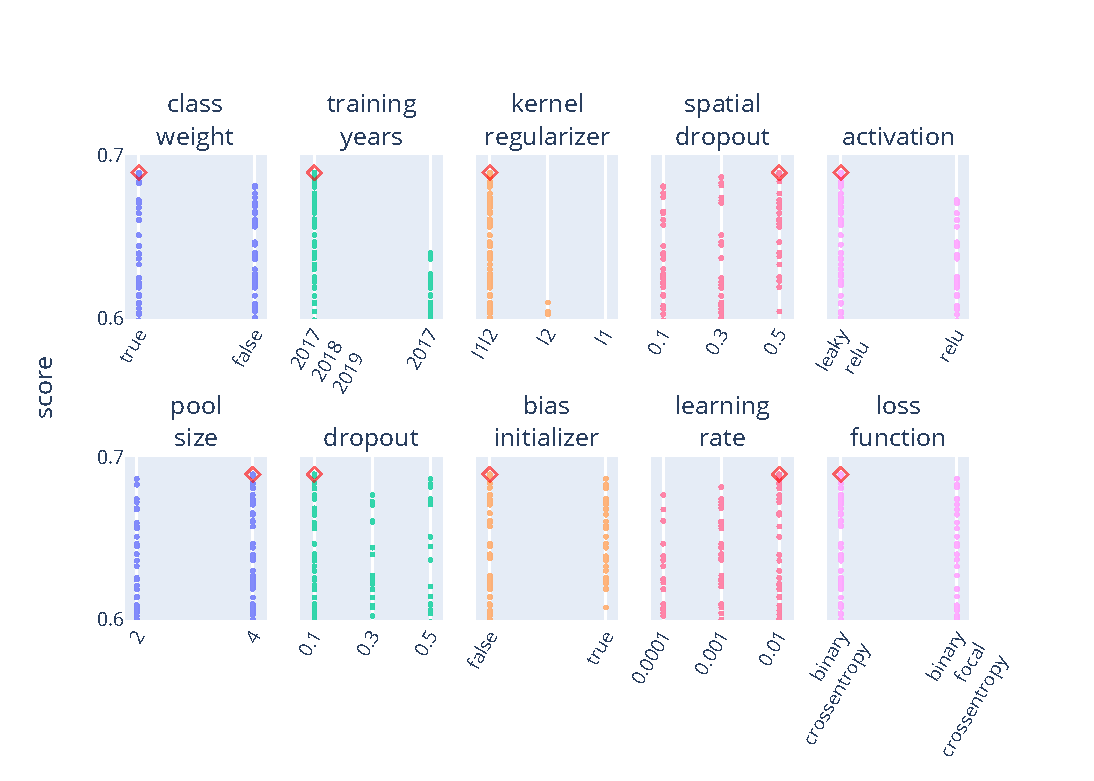
\includegraphics[width=0.9\linewidth, trim={10pt 10pt 40pt 40pt}, clip]{figures/figures_tuner/hyperband_resnet_params.pdf}
    \caption{The top f2-scores for the initial hyperparameter tuning process are highlighted, with the best score marked by a diamond shape.}
    \label{fig:hyperband_resnet_params}
\end{figure}

In the most successful trial, the model utilized training data from the medians of 2017, 2018, and 2019, applied L1L2 kernel regularization, used a spatial dropout rate of 0.5, and employed Leaky ReLU activation. The pool size was set to 4, dropout to 0.1, and bias initialization was disabled. The learning rate was 0.01, and the loss function was binary crossentropy, resulting in a score of 0.69.

While some of the initial trial's hyperparameters do not show significant overall improvement, some parameters do stand out. This is illustrated in Fig.\,\ref{fig:hyperband_resnet_params}, particularly regarding training years, kernel regularization, activation function, and learning rate.

\section{Model Architecture}

\begin{figure}[ht]
    \centering
    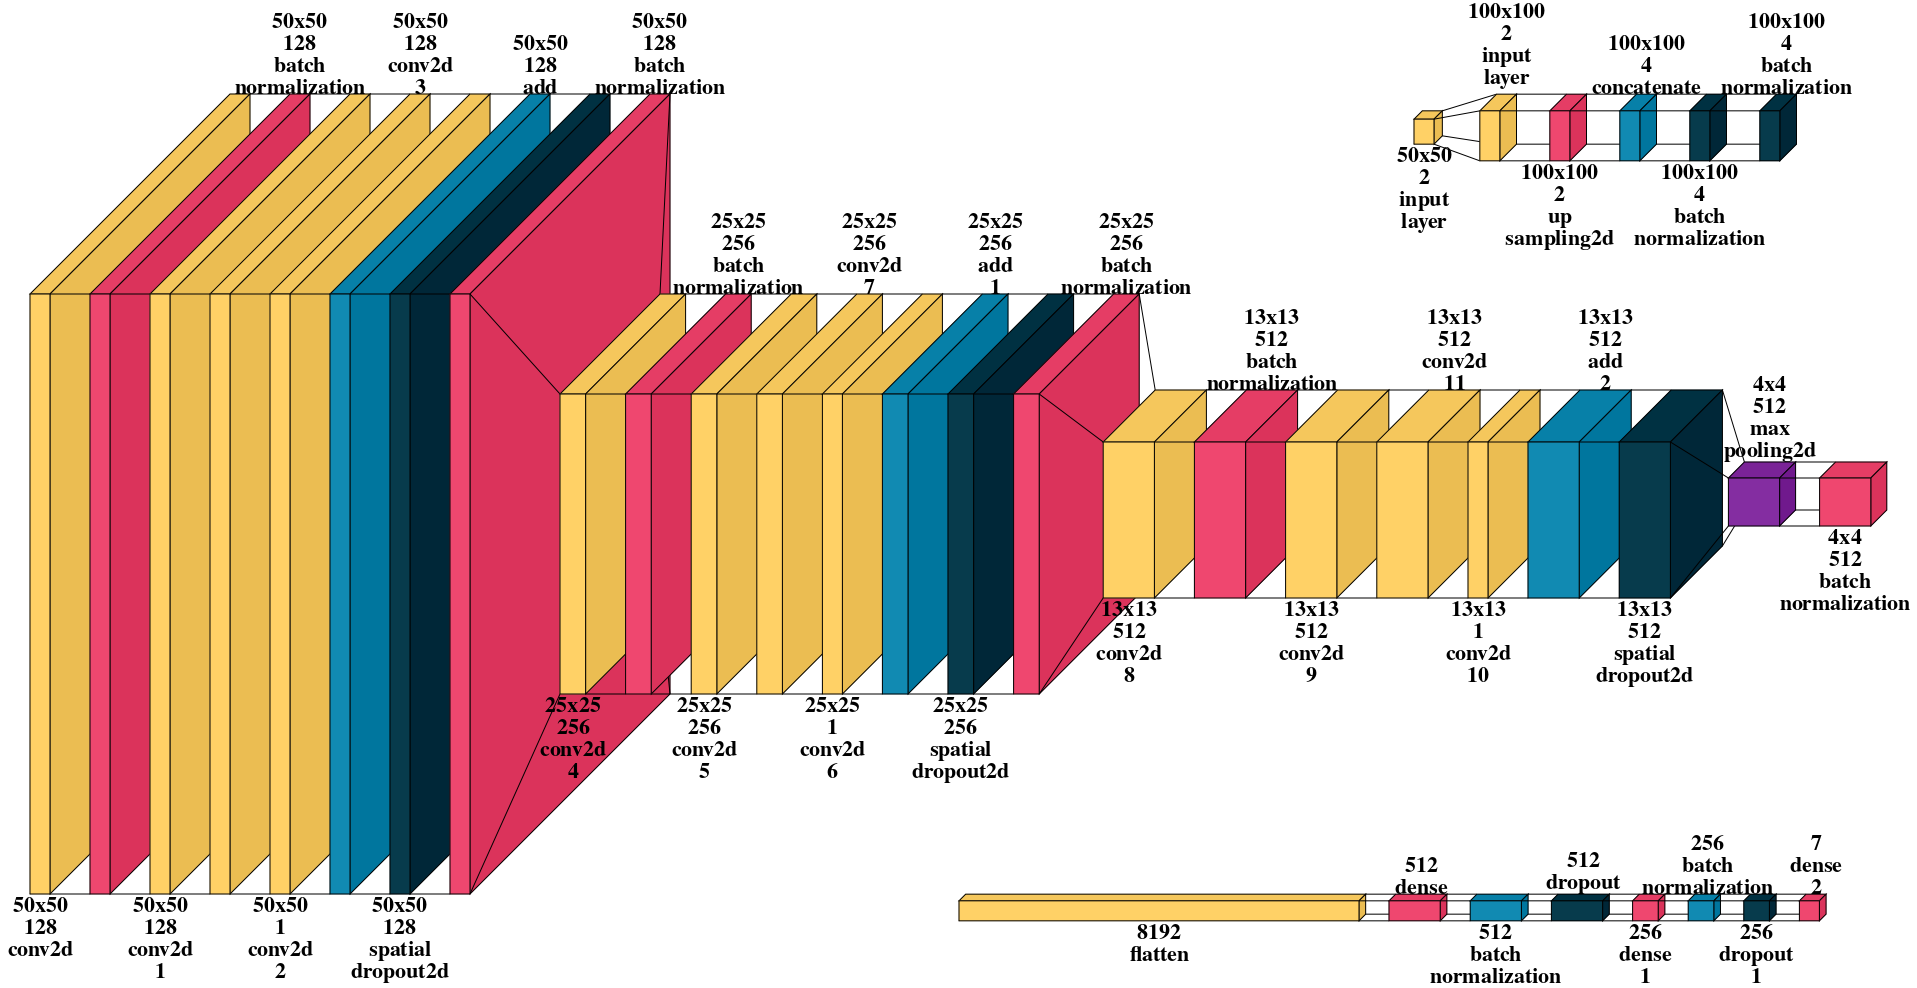
\includegraphics[width=0.9\linewidth]{figures/figures_tuner/model_layered_view.png}
    \caption{The model's layered architecture is depicted. The top-right shows the input layers, the middle section displays the convolutional layers, and the bottom-right illustrates the fully-connected layers. The layered views were generated using VisualKeras (\cite{visualkeras}).}
    \label{fig:model_layered_view}
\end{figure}

Fig.\,\ref{fig:model_layered_view} illustrates the detailed architecture of the deep learning model, highlighting the flow of data through its various layers. The model starts with input layers, which include upsampling layers to handle inputs with different dimensions. This ensures that all input sources are properly aligned for processing within the model. The network then progresses through multiple convolutional layers, with filter sizes generally increasing as the layers deepen. Batch normalization and dropout layers are strategically placed to regularize the model and prevent overfitting.

The architecture incorporates residual connections for maintaining gradient flow during backpropagation. These connections enable the network to be deep without suffering from issues like vanishing gradients, as highlighted in \cite{resnet}. As the network advances, spatial dimensions are reduced through pooling and striding operations, leading to a flattening layer that prepares the data for the fully connected (dense) layers. These dense layers further reduce the dimensionality, eventually outputting a 7-dimensional vector corresponding to the classification into 7 different tree genera, aligning with the model's goal of predicting tree types.
